\chapter{Ogólny opis systemu}
\label{cha:wprowadzenie}


\section{Cel (przeznaczenie) systemu}
\label{sec:celePracy}

Celem systemu automatyczny parking jest umożliwienie komputerowej obsługi pobierania opłat za~pozostawienie pojazdu na parkingu na określony czas. System rozpoznaje ze zdjęcia tablice rejestracyjne pojazdów i na tej podstawie umożliwia wjazd samochodów na parking, a także opuszczenie go.

\section{Udziałowcy i użytkownicy}

\begin{list}{$\bullet$}{}
\item Właściciel - posiada parking, jest kierownikiem zarządzającym pracownikami, system prezentuje mu zebrane statystki
\item Klient - osoba, która korzysta z usług automatycznego parkingu i wjeżdza samochodem na jego teren
\item Operator - osoba kontrolująca parking w danej chwili, w przypadku błędów, przegląda zarejestrowane zdjęcia i poprawia czas wjazdu i wyjazdu

\end{list}

\section{Podstawowe cele udziałowców i użytkowników}

\begin{table}[H]
	\begin{tabular}{|l|l|l|} \hline
	\textbf{Udziałowcy}	& \textbf{Cel} & \textbf{Priorytet} \\ \hline% \bottomrule
	Klient	& Wjechanie na parking & Wysoki \\
	Klient	& Opuszczenie parkingu & Wysoki \\
	Klient	& Wpisanie numeru rejestracyjnego & Wysoki \\
	Klient	& Potwierdzenie zdjęcia & Wysoki \\
	Klient	& Anulowanie wpisanego numeru rejestracyjnego & Średni \\
	Klient	& Uiszczenie opłaty & Wysoki \\
	Operator& Przeglądanie zdjęć & Średni \\
	Operator& Poprawa czasu wjazdu i wyjazdu w bazie & Średni \\
	Właściciel& Wyświetlenie statystyk & Niski \\ \hline
	\end{tabular}
\end{table}

%płatność kartą i gotówką?
W~aktualnym systemie klient podjeżdża do terminala, naciska przycisk i~odbiera bilet z godziną wjazdu. Przy opuszczaniu parkingu wkłada otrzymany przy wjeździe bilet i~dokonuje opłaty.
W~naszym systemie klient, wjeżdżając na parking, nie musi podjeżdżać do terminala i~czekać na wydrukowanie kartki z~godziną wjazdu. System zrobi zdjęcie tablicy rejestracyjnej i~sam otworzy szlaban. W~ten sposób oszczędzany jest papier oraz tusz. Operator nie musi dbać o~to żeby ich nie zabrakło. Musi jedynie interweniować w~przypadku oszustwa.


\section{Granice systemu}
\begin{figure}[H]
	\centering
	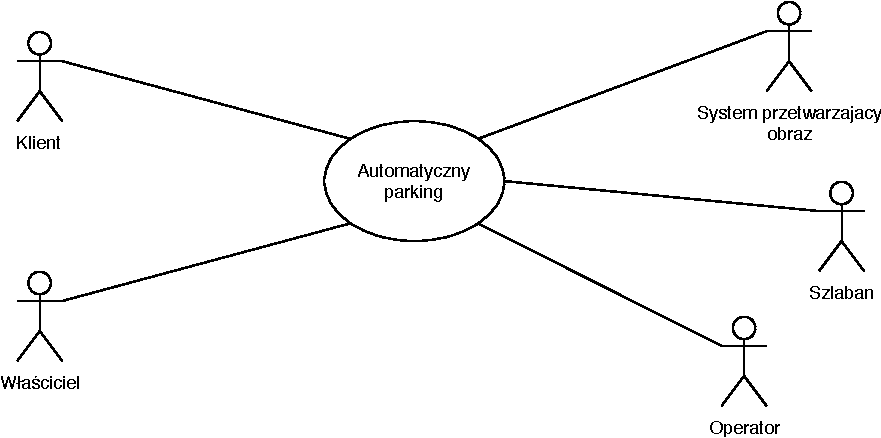
\includegraphics[width=90mm]{diagramy/graniceSystemu.pdf}
	\caption{Granice systemu automatyczny parking \label{overflow}}
\end{figure}

\section{Lista funkcji systemu}


% Diagram czynności: Klient wjeżdża na parking
\begin{figure}[H]
	\centering
	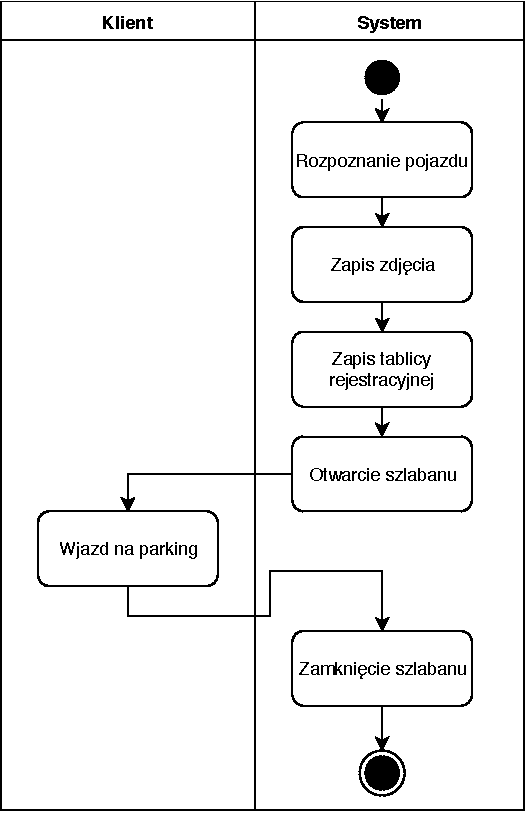
\includegraphics[width=90mm]{diagramy/DiagCzynWjazd.pdf}
	\caption{Diagram czynności: Klient wjeżdża na parking \label{overflow}}
\end{figure}


% Diagram czynności: Klient opuszcza parking
\begin{figure}[H]
	\centering
	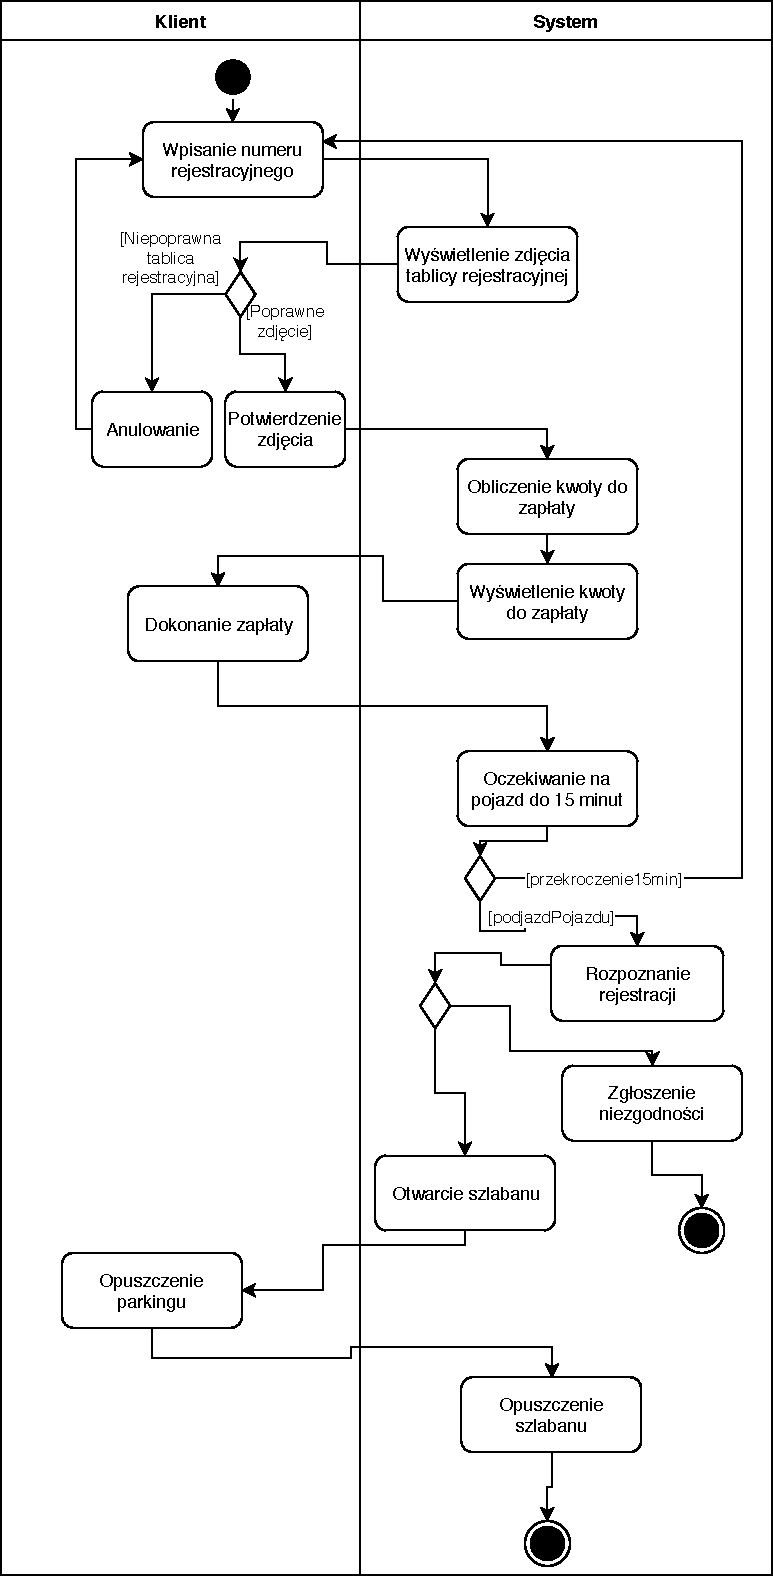
\includegraphics[width=90mm]{diagramy/DiagCzynWyjazd.pdf}
	\caption{Diagram czynności: Klient opuszcza parking \label{overflow}}
\end{figure}


% Diagram czynności: Operator weryfikuje wykryte oszustwo
\begin{figure}[H]
	\centering
	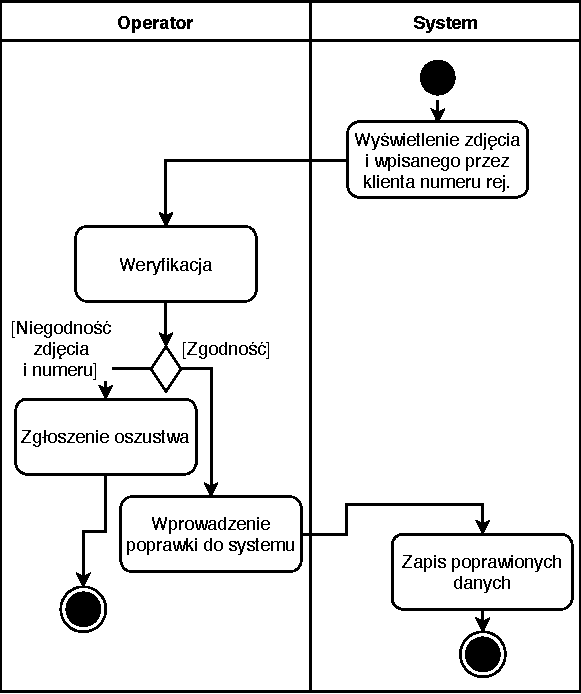
\includegraphics[width=90mm]{diagramy/DiagCzynWyswietlZdjecia.pdf}
	\caption{Diagram czynności: Operator weryfikuje wykryte oszustwo \label{overflow}}
\end{figure}

% Diagram czynnosci: Właściciel wyświetla statystyki
\begin{figure}[H]
	\centering
	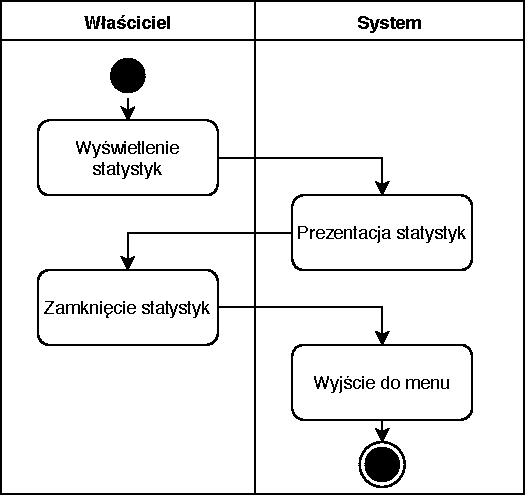
\includegraphics[width=90mm]{diagramy/DiagCzynStatystyki.pdf}
	\caption{Diagram czynności: Właściciel wyświetla statystyki \label{overflow}}
\end{figure}




